Para corregir el factor de potencia (es decir buscar que su valor se aproxime lo más que se
pueda a 1), se debe agregar un elemento reactivo que compense el desfasaje entre la
tensión y la corriente producido por la carga conectada a la red. En el caso de este trabajo práctico, la carga es inductiva (balastro), por este motivo se debe agregar un condensador que se conectará entre los puntos A y B del esquema de la figura \ref{fig:exp1med}.

El valor de capacitancia necesario se calcula utilizando la expresión \ref{eq:corrFp} del marco teórico, y a partir de las mediciones obtenidas en el primer experimento:

\begin{equation*}
    C=\frac{P\cdot \tan\phi}{V^2\cdot \omega}=\frac{32.32[W]\cdot 2.426}{220^2 \cdot 2\pi \cdot50 [Hz]} = 4.679 [\mu F]
\end{equation*}


En el laboratorio había disponibles una serie de capacitancias \textit{shunt} utilizadas para la compensación de $\mathrm{fp}$. El valor más cercano disponible fue de una $C=4 [\mu F]$. 

Una vez conectado el capacitor en los terminales correspondientes, se volvió a visualizar las formas de onda de los puntos C1 y C2 en el osciloscopio, esperando que ahora el desfasaje se haya corregido. El visor del osciloscopio se muestra en la figura \ref{fig:corrFp}

\begin{figure}[H]
    \centering
    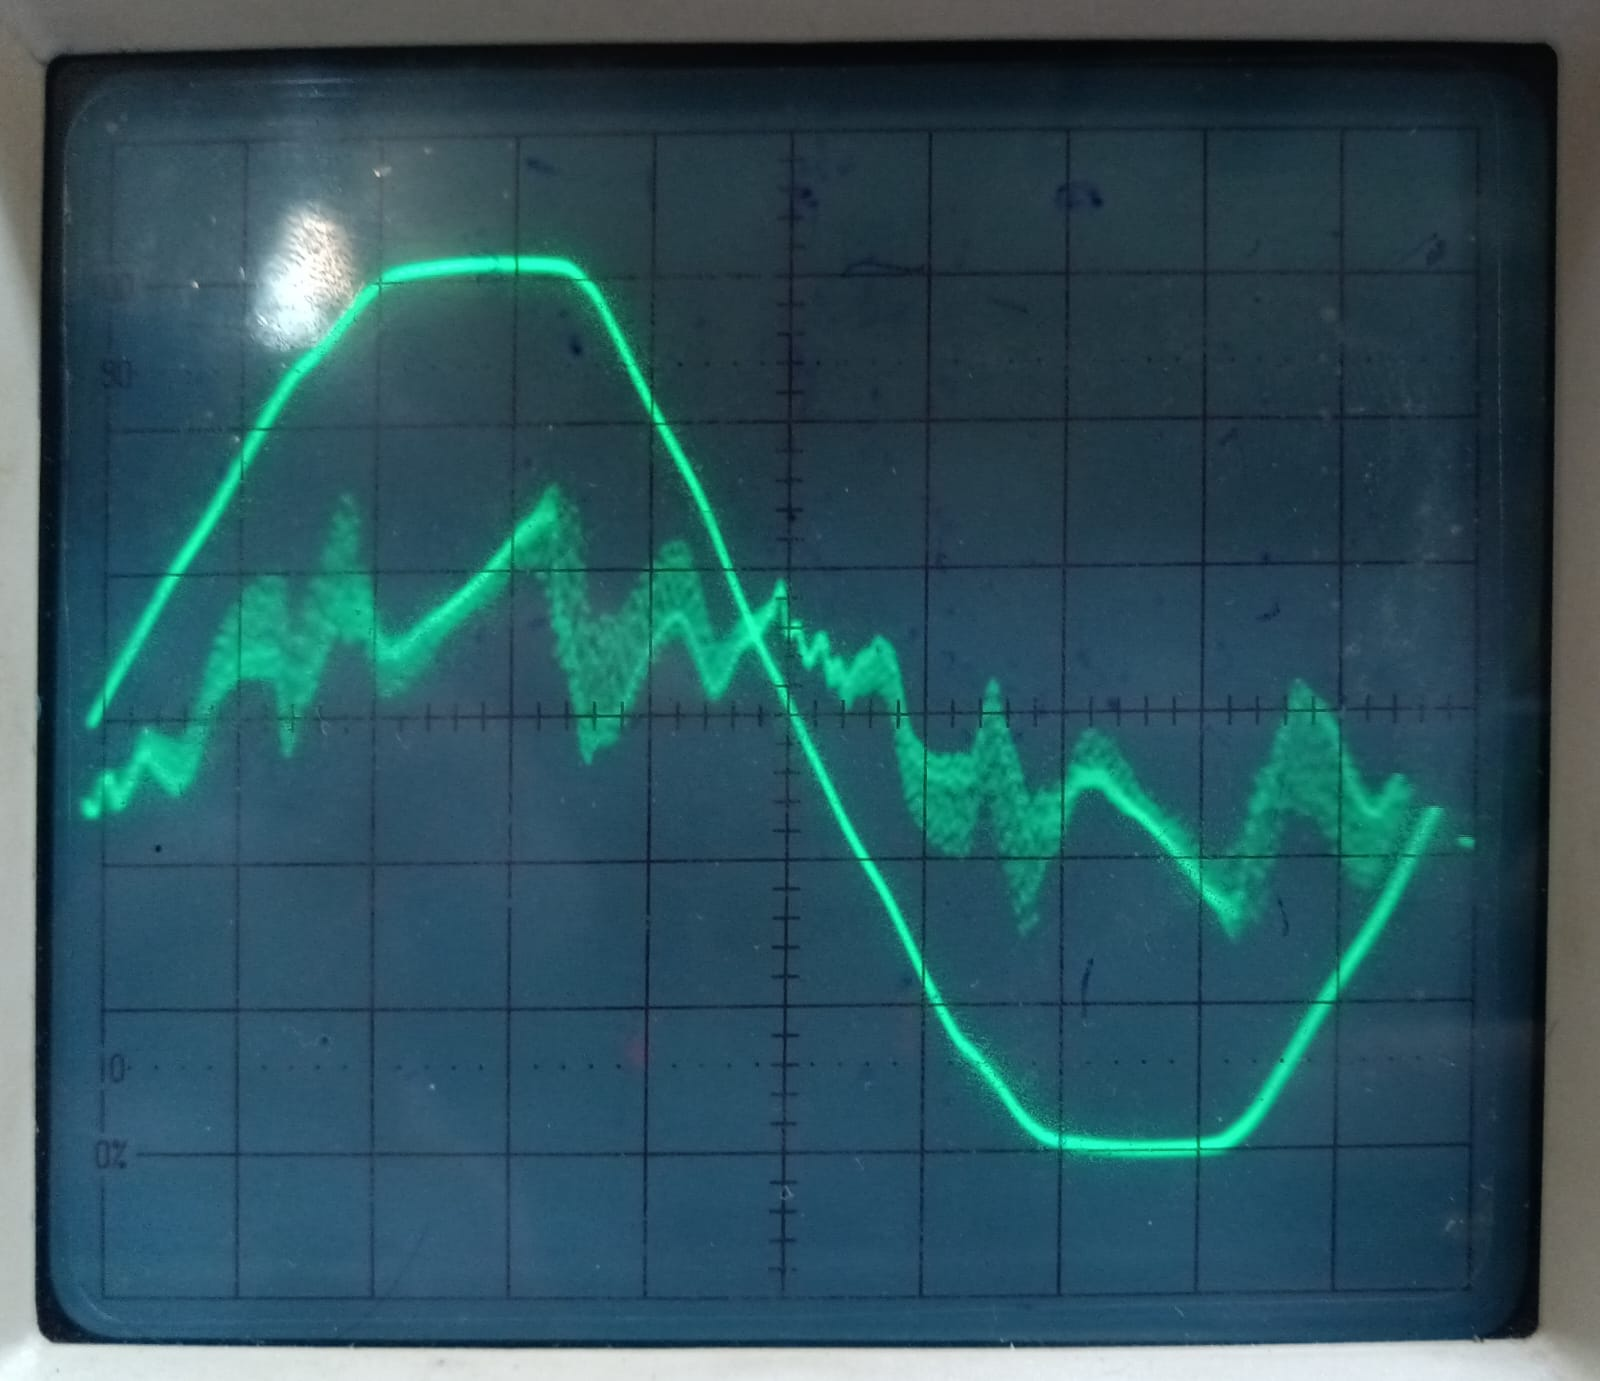
\includegraphics[width=0.6\linewidth]{Imagenes/Mediciones/corrFp.jpeg}
    \caption{Factor de potencia corregido}
    \label{fig:corrFp}
\end{figure}

Se observa que si bien el desfasaje se ha corregido, y el factor de potencia se acercó bastante a 1, la forma de onda se vio bastante afectada. Esto sucede porque las formas de onda presentes en
la red de alimentación siempre están deformadas por acción de las diferentes cargas
conectadas a la misma.
Estas deformaciones incluyen las que se originan en los efectos de saturación de los
transformadores y del ruido por conmutación de una múltiple variedad de equipos o dispositivos eléctricos. 

Se procedió a medir nuevamente el valor de la potencia aparente a partir de las mediciones de la tensión y corriente (de la misma manera que en el experimento 1). Los resultados fueron:

\begin{align*}
    V &= 230 [V]\\
    I &= 0.131 [A]\\
    S &= 30.121 [VA] \\
\end{align*}


Como era de esperarse, el valor de la potencia aparente $S$ se redujo hasta volverse casi equivalente a la potencia activa $P$. Lo cual implica indefectiblemente una mejora en el rendimiento: 

\begin{equation*}
    \mathrm{fp} = \frac{P}{S} = \frac{32.32}{30.121} \approx 1
\end{equation*}